\begin{frame}{Multi-hop}
\framesubtitle{What ?}
\begin{columns}
\begin{column}{0.6\textwidth}
\begin{itemize}
    \item Message relayed to neighbor
    \item Range increased
    \item Power efficient for border nodes
    \item Adapt to topology
    \item Overall higher energy consumption
\end{itemize}
\end{column}
\begin{column}{0.4\textwidth}
\begin{figure}[H]
    \centering
    \begin{tikzpicture}[auto, thick]
      % Place super peers and connect them
      \foreach \place/\name in {{(0,0)/a}}
        \node[gateways] (\name) at \place {};
      \node[motes] (a4) at (-2, 1) {};
      \node[motes] (a5) at (-3, 1.3) {};
      \node[motes] (a7) at (-2.5, -0.5) {};
      \node[motes] (a8) at (-2, -1) {};
     \foreach \pos/\i in {below left of/1, below of/2, left of/3, above left of/6}
        \node[motes, \pos =a ] (a\i) {};
      \foreach \speer/\peer in {a/a1,a/a2,a/a3,a7/a3,a8/a3}
        \path[dotted] (\speer) edge (\peer);
      \path[dotted,->] (a5) edge (a4);
      \path[dotted,->] (a4) edge (a6);
      \path[dotted,->] (a6) edge (a);
    \end{tikzpicture}
    \caption{Multi-hop Communication\label{fig:multihop}}
\end{figure}
\end{column}
\end{columns}
\end{frame}

\begin{frame}{Multi-hop}
\framesubtitle{LoRaWAN Extension}
% \begin{columns}
% \begin{column}{0.3\textwidth}
% \end{column}
% \begin{column}{0.7\textwidth}
% \end{column}
% \end{columns}
\begin{figure}[H]
    \centering
    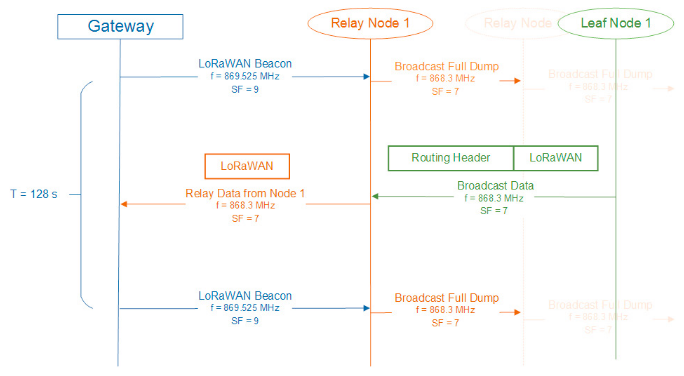
\includegraphics[width=0.98\textwidth]{presentation.tex/fig/lorawanextension.png}
    \caption{LoRaWAN Extension\footnotemark}
\end{figure}

\footcitetext{DIAS2018424}
\end{frame}

\begin{frame}{Multi-hop}
\framesubtitle{Linear Sensor Network}
\begin{columns}
\begin{column}{0.5\textwidth}
\begin{figure}[H]
    \centering
    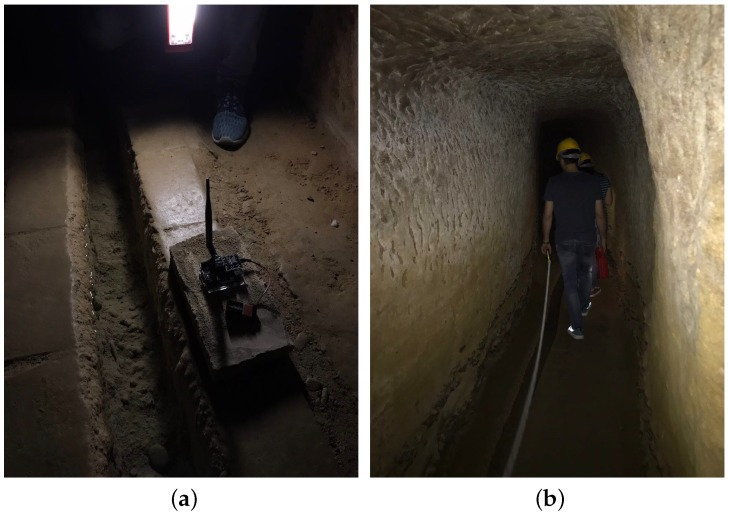
\includegraphics[width=1\textwidth]{presentation.tex/fig/lsnlora.jpg}
    \caption{Underground tunnel installation\footnotemark}
\end{figure}
\end{column}
\begin{column}{0.5\textwidth}
\begin{figure}[H]
    \centering
    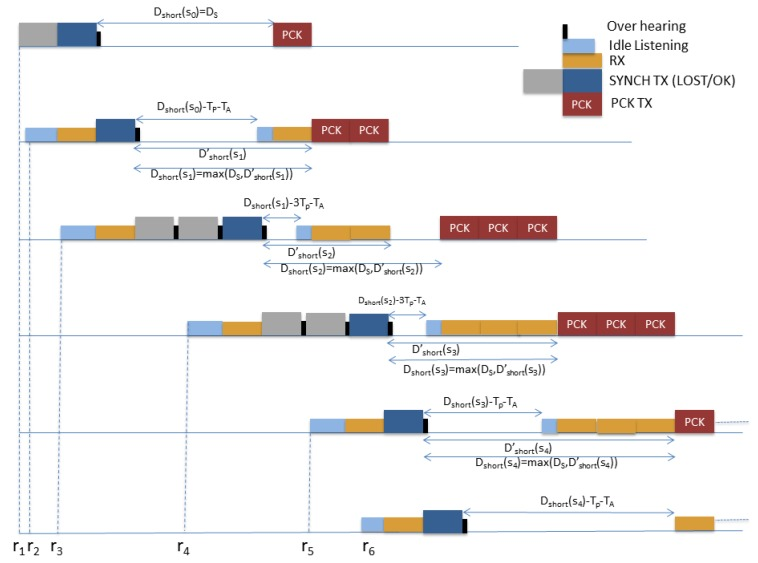
\includegraphics[width=0.98\textwidth]{presentation.tex/fig/lsnlora2.jpg}
    \caption{Protocol\footnotemark}
\end{figure}
\end{column}
\end{columns}
\footcitetext{Abrardo_2019}
\end{frame}



\begin{frame}{Multi-hop}
\framesubtitle{LoRaBlink}
\begin{columns}
\begin{column}{0.3\textwidth}
\begin{figure}[H]
    \centering
    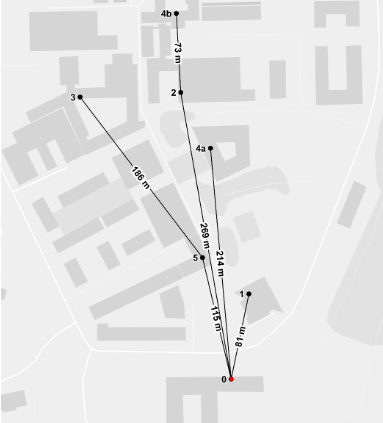
\includegraphics[width=1\textwidth]{presentation.tex/fig/lorablink2.png}
    \caption{Range\footnotemark}
\end{figure}
\end{column}
\begin{column}{0.7\textwidth}
\begin{figure}[H]
    \centering
    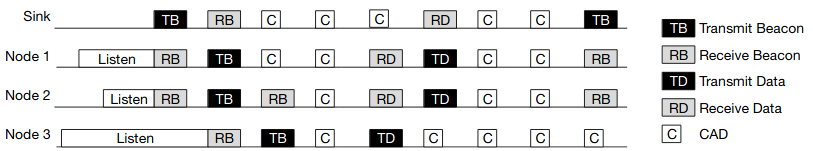
\includegraphics[width=0.98\textwidth]{presentation.tex/fig/lorablink.png}
    \caption{LoRaBlink protocol\footnotemark}
\end{figure}
\end{column}
\end{columns}
\footcitetext{lorablink}
\end{frame}


\begin{frame}{Multi-hop}
\framesubtitle{LoRa Multi-hop Network}
% Sum up of multi-hop LoRa
% What related work achieved
\begin{itemize}
    \item Cope with collision through
    \begin{itemize}
        \item Node coordination
        \item Clock synchronization
    \end{itemize}
    \item Cope with bordering nodes through
    \begin{itemize}
        \item Increased range
    \end{itemize}
    \item Linear Sensor Network
    % \item Interference resilience
\end{itemize}
\end{frame}

\begin{frame}{Multi-hop}
\framesubtitle{LoRa Multi-hop Network}
% My work what it will achieve based on that
\begin{itemize}
    \item Low-power
    \begin{itemize}
        \item Time-Division
        \item Synchronization
        \item Scheduling
    \end{itemize}
    \item Reliable
    \begin{itemize}
        \item No collision
        \item Interference resistance
        \item Frequency-Division
    \end{itemize}
    \item Bi-directional
\end{itemize}
\end{frame}
